\chapter{Act II}



\begin{figure}
   \centering
   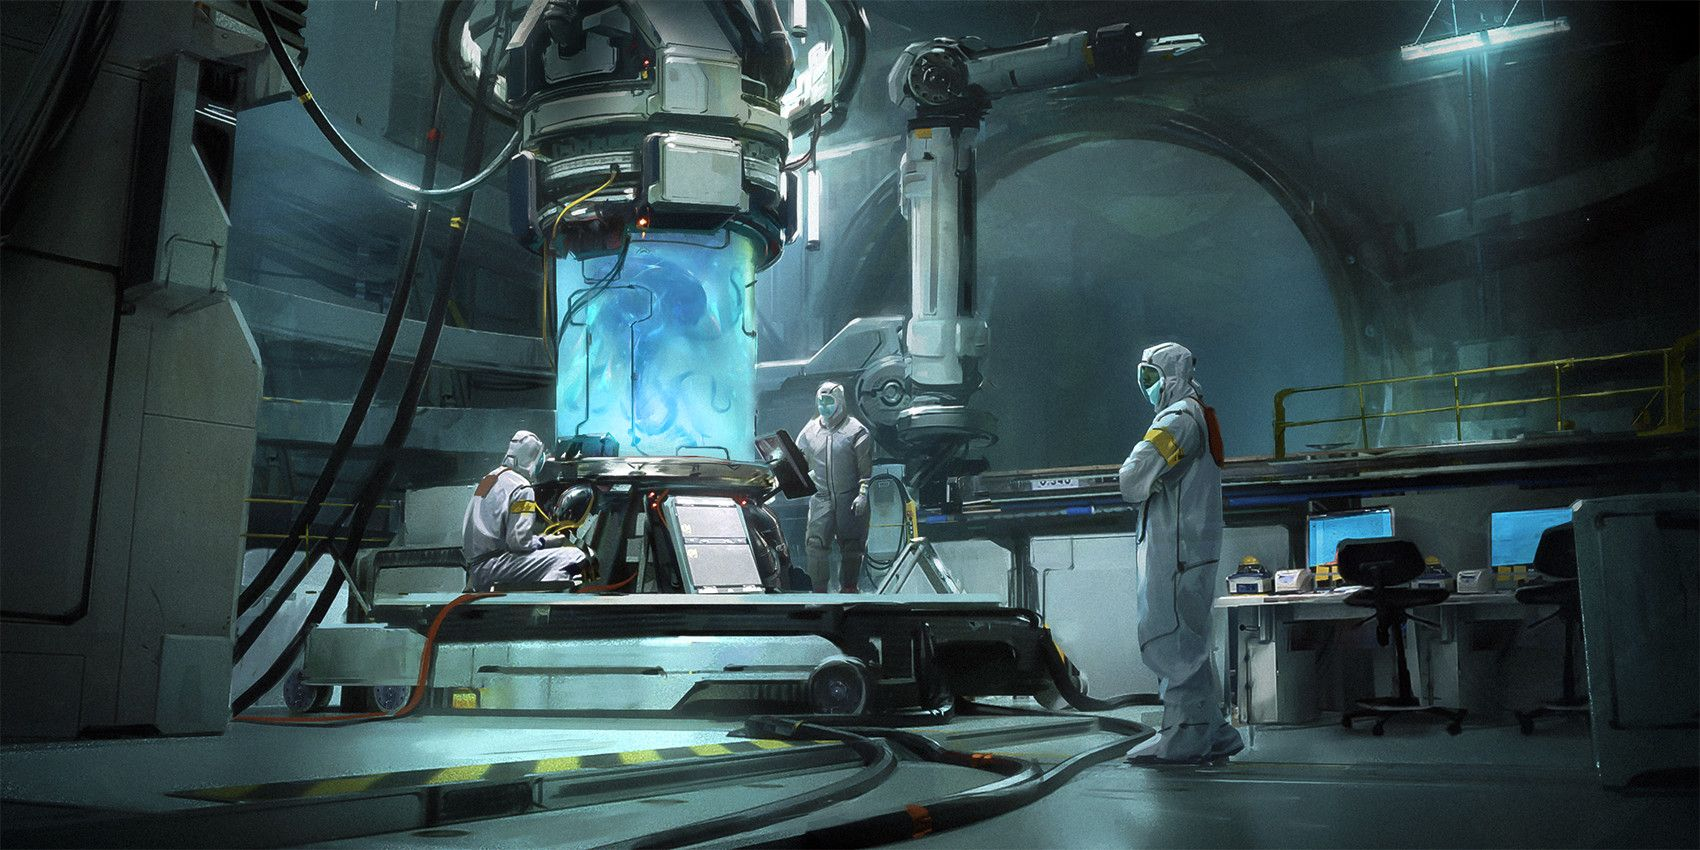
\includegraphics[width=1.0\textwidth]{img/bg/lab.jpg}
\end{figure}


\section{Where the hell is the body?}


\begin{rpg-commentbox}{The Alien}
   The creature controls the host to seek a dark and quiet place where it can grow stronger eventually reaching stage II.

    
    \medskip

    If the PCs had killed the first alien, just have some other prisoners infected (remember that there were more spores)
    and describe gore bodies as they walk through the refinery
\end{rpg-commentbox}




\newsect

\section{Escape plan}


\begin{rpg-commentbox}{Protect Kathia}
    Ideally, Kathia has left her corporate card in a biometric safe, so her protection is paramount to any escape plan.

    Mageed contacts prisoners via intercom and says that the crew is working on a escape plan. They will use Kathia's ship and for that, they need to bypass the lockdown.
    Prisoners are asked to gather enough mining explosives and bring them to the reactor core at the refinery. A handful of explosives can damage the reactor and cut power in the station, that will deactivate the lockdown. However, prisoners will need EVA suits as the air in the station will soon deplenish.
 \end{rpg-commentbox}


 \begin{rpg-commentbox}{Grab Explosives at the mine}
    Depending how players go fetch the mining explosives, they will face the alien fully morphed to stage 2. \textbf{Alien has stats of a Xenomorph stalker}

    Run a stealth mode scene moving some of the players through the mines. \textbf{mobility} vs \textbf{observation}
 \end{rpg-commentbox}


 
 \begin{rpg-commentbox}{Bring explosives to reactor}
    At this point in time, if one of the larva is still alive and the PCs did not encounter it, people will hear agonizing screams as the larva infects a new host. 

    Something cool for this one is to let the host have a welding torch. The alien won't use it but it hangs in a loosely held bandoleer making a lot of noise while the exo-parasite walks the refinery. This can make for some interesting scenes as for example, players setting the explosives in the reactor core while listening to the crackling sound of metal against the crate floor.

    Players must hack the reactor door \textbf{comtech}, put the explosives and set a controlled explosion. Failures might bring nice complications
 \end{rpg-commentbox}

 \begin{rpg-commentbox}{Load cargo elevator with sulfuric acid}
    Needed to crack safe open without corrupting the corporate card

    Players must use crane to pick acid containers \textbf{heavy machinery}
 \end{rpg-commentbox}


 \begin{rpg-commentbox}{Other options}
   These are overall suggestions. Adapt the scenario to your liking.
\end{rpg-commentbox}

 \newsect

 \section{What is happening upstairs?}
 
\begin{rpg-commentbox}{We've got a situation here}
   From time to time Mageed gets in the intercom and give instructions. At some point, let him say hang-on, we got a situation here. All communications after this only return hiss static. Increase stress level by 1.
\end{rpg-commentbox}

\begin{rpg-commentbox}{End of Act}
   \textbf{Act 2 ends when prisoners leave prison ward.}
\end{rpg-commentbox}